\chapter{Metodologia}
\label{cap:metodologia}

\section{Objetivos}
O objetivo geral deste trabalho é realizar uma análise da API do sistema Android a partir de uma análise estática de seu código fonte, e então avaliar a possibilidade de utilizar os resultados como referência para o desenvolvimento de aplicativos desenvolvidos para o Android, partindo da premissa que os aplicativos desenvolvidos utilizando a API do sistema são fortemente dependentes da mesma.

A partir da análise do código fonte, definir intervalos para valores da métrica que se adequam a arquitetura do sistema, assim como definir intervalos para os aplicativos do sistema e verificar o grau de aproximação que ambos encontram em seu design. Verificar então a possibilidade da validação dos intervalos de valores através de regressão polinomial utilizando métricas OO em função de métricas de tamanho.

Assumindo que o código da API do sistema possui uma boa arquitetura, propomos um fator de aproximação para aplicar a aplicativos em desenvolvimento para avaliar sua qualidade de acordo com a aproximação ao sistema, em termos de métricas estáticas de código. Essas métricas utilizadas refletem complexidade arquitetural e decisões de design, essencialmente métricas OO.

Esse fator de aproximação a nível de software é centralizado em 0, onde valores positivos indicam valores das métricas maiores que os da API, e valores negativos indicam resultados menores que os da API. Quanto mais próximo de 0, mais próximo a API, e quanto menor o valor, melhores são os resultados. Usar esse score como forma de avaliar a qualidade em comparação com a API, julgando então como resultados teóricos melhores, próximos a API, ou piores, para valores negativos, próximos ao 0, e positivos, respectivamente.

%É importante incluir métricas que refletem o volume de código para dar resultados relativos ao tamanho do aplicativo sendo avaliado, uma vez que várias métricas tem seu valor de referência variável de acordo com o tamanho do código. Utilizar valores do sistema, como milhões de linhas de código, como referência para analisar um aplicativo com apenas algumas centenas de linhas resulta em uma comparação inválida para os valores de algumas métricas, como discutido no Capítulo~\ref{cap:metricas}.

Algumas conclusões talvez já possam ser tiradas de acordo com a aproximação do código do sistema\footnote{``Código do sistema'' está sendo utilizado para referenciar a API de desenvolvimento de aplicativos} aos aplicativos nativos. Se a média de scores indicar um valor negativo, por exemplo, indica que na média os aplicativos do sistema tem valores teóricos melhores que os da plataforma, e talvez o objetivo de um novo \textit{app} seja se manter dentro dos intervalos de valores do sistema, mas tentando ficar com valores ainda menores, não necessariamente iguais aos da API. Essa verificação de scores é reflexão dos intervalos de valores que serão definidos no Capítulo~\ref{cap:resultados}, e será discutida no mesmo capítulo.

\section{Questão de pesquisa e hipóteses}

Baseando-se nas ideias apresentadas, é levantada a seguinte questão de pesquisa (QP):

\begin{itemize}
%\item QP - É possível monitorar métricas estáticas de código fonte de aplicativos Android de acordo com a análise e predição da evolução do código do sistema?
\item QP - É possível monitorar métricas estáticas de código fonte de aplicativos Android de acordo com a análise de intervalos e aproximação do código do sistema?
%\item É efetivo usar o próprio sistema como arquitetura referência devido ao acoplamento de aplicativos com a própria API de desenvolvimento?
\end{itemize}

Respondendo a essa pergunta podemos confirmar a efetividade de utilizar o próprio sistema como arquitetura referência em análise de aplicativos desenvolvidos para ele. Para alcançar os objetivos descritos e responder a questão de pesquisa que foi definida, algumas hipóteses devem ser estudadas e avaliadas:

\begin{itemize}
\item H1 - É possível identificar padrões e tendências na evolução da arquitetura do sistema Android e nos aplicativos desenvolvidos para ele.
\item H2 - O desenvolvimento de aplicativos Android pode ser guiado pelo resultado de uma análise evolutiva do código do próprio sistema.
\item H3 - Uma grande aproximação ao sistema implica em uma boa qualidade de código.
\item H4 - As decisões arquiteturais teóricas aplicadas no estudo de caso e-lastic estão relacionadas com decisões arquiteturais baseadas em métricas.
\end{itemize}

A hipótese H1 será testada com a identificação manual de um comportamento de métricas no código fonte de diversas versões do sistema. O objetivo principal dessa hipótese é identificar se o sistema contém algum padrão nos valores das métricas ao longo de sua evolução, ou se os valores são completamente diferentes das demais versões e portanto não relacionados. A identificação de um padrão de permanência/aumento/diminuição nos ajuda a definir intervalos bons de métricas válidos para o sistema, e ter uma ideia se eles continuarão válidos para versões futuras.

H2 é tratada com análise do código fonte da API e dos aplicativos, identificando semelhança entre ambos. Identificando semelhanças entre ambos, podemos confirmar algumas premissas como o alto acoplamento entre API e aplicativos, que já é esperado como outros trabalhos já sugerem. Essa confirmação nos leva a afirmar que os valores de métricas para o sistema, já mais consolidado, podem ser referência para comparação direta com aplicativos sem preocupação com escala do projeto, podendo ser utilizados durante desenvolvimento de aplicativos para Android.

H3 parte da ideia de que, caso a API tenha bons valores de métricas, o que será verificado no Capítulo~\ref{cap:resultados}, e portanto boa qualidade de código fonte, uma aproximação de aplicativos em relação à API em termos de métricas indica uma boa qualidade de código fonte. Para avaliar essa hipótese, verificaremos os resultados da proposta de cálculo de semelhança de aplicativos que será discutida também no Capítulo~\ref{cap:resultados}.

Para a Hipótese H4, será avaliado, através da comparação com o sistema, o resultado parcial inicial deste trabalho, que corresponde a um aplicativo Android (descrito no Apêndice~\ref{ap:elastic}) desenvolvido com o objetivo de criar uma arquitetura modularizada, flexível e manutenível. Foram tomadas diversas decisões teóricas com o objetivo de alcançar a melhor arquitetura para um aplicativo Android, desenvolvido para um estudo de caso específico, e então desejamos avaliar se essas decisões tomadas, com base em experiência de desenvolvedor e padrões de projeto, são semelhantes às decisões que podem ser tomadas com base em resultados de análise estática de código fonte, como as análises realizadas neste trabalho.

\section{Trabalhos relacionados}

\citeonline{androidblackberry}  realiza um estudo de dependência das APIs de desenvolvimento tanto da plataforma Android quanto da plataforma Blackberry, a fim de fazer uma comparação entre os sistemas. A partir disso, é verificado o quanto uma API influencia na quantidade de código desenvolvido, assim como é verificada a dependência de código de terceiros para o desenvolvimento de aplicativos. Em suma, o resultado comparativo demonstrou que aplicativos no sistema Android são significativamente mais dependentes da API do sistema devido a maior completude da API, reduzindo por consequência a quantidade de código de terceiros e código próprio dentro dos projetos. Embora possa tornar mais fácil o desenvolvimento, essa dependência maior em relação ao código do sistema torna o código de aplicativo desenvolvido para Android difícil de ser portado para outras plataformas.

\citeonline{samoa} apresenta o desenvolvimento de uma ferramenta de análise estática de código, que avalia não apenas métricas de código fonte, mas também a dependência de código de terceiros dentro do projeto de aplicativos Android. O objetivo desse trabalho não foi apenas analisar software em plataforma móvel, mas também diferenciar a abordagem quado analisando um software tradicional ou um software para dispositivo móvel, de forma a verificar a manutenibilidade desses sistemas. O estudo de \citeonline{androidblackberry} também apresenta algumas discussões no quesito manutenibilidade em sistemas móveis. Assim como neste último, \citeonline{samoa} demonstra uma alta dependência de aplicativos Android em relação ao sistema, apresentando em geral cerca de  2/3 das chamadas de método de aplicativos sendo para bibliotecas externas ao app, em sua maioria para a API Android ou métodos de bibliotecas padrão Java.

\citeonline{evolutionandroid} reforça a ideia de dependência de aplicativos em relação a API Android, e fala sobre as grandes mudanças da API devido a sua rápida evolução nos ultimo anos. Tenta então ajudar desenvolvedores com dicas para melhor se prepararem para mudanças na plataforma, assim como para mudanças em bibliotecas de terceiros, que podem ser bastante significativas em diversos aspectos, e consequentemente impactar negativamente no desenvolvimento de aplicativos, introduzindo mudanças bruscas e possivelmente bugs.

A dependência dos aplicativos Android em relação ao próprio sistema fica bem clara em vários trabalhos publicados até a data de escrita deste trabalho, o que motiva bastante a coleta e análise de métricas no sistema para serem comparadas com métricas de aplicativos. Os resultados podem ser bastante úteis para novos desenvolvedores que não têm referências para basear seu desenvolvimento e poderiam guiar a evolução de seu sistema em comparação com a evolução do próprio Android.

Em se tratando de métricas, \citeonline{predictivemodels} apresenta várias abordagens para analisar métricas em software, mais a nível de projeto, e gerar modelos preditivos. Vários métodos de aprendizado de máquina são explanados e comparados em termos de modelagem relacionada a métricas em software. 

\citeonline{evaluatingpredictivemodels} descreve uma comparação de várias técnicas para prever qualidade de código, classificando como alto risco, com grande probabilidade de conter erros, ou baixo risco, com probabilidade de conter poucos ou nenhum erro. Vários métodos são avaliados desde regressão até redes neurais. Embora os resultados apresentados no artigo não tenham sido muito promissores, a conclusão de que nenhum dos métodos utilizados se mostrou efetivo para separar entre componentes com ou sem erros pode ajudar a remover algumas tentativas desnecessárias em trabalhos relacionados.

Ainda tentando avaliar a probabilidade de conter erros, \citeonline{validationmetricsfaultprediction} também utiliza técnicas de \textit{machine learning}, utilizando como dados essencialmente métricas para sistemas orientados a objetos, de Chidamber e Kemerer. Esse estudo é conduzido em cima de software livre, utilizando como estudo de caso o Mozilla. Uma das contribuições que o artigo apresenta é relacionar classes e bugs reportados dentro do Mozilla. Além disso, verificaram que a métrica de acoplamento entre objetos (\textit{coupling between objects} - CBO) foi a mais determinante em prever probabilidade de falha em classes, refletindo um pouco da qualidade do código escrito. Da mesma forma, a métrica linhas de código (\textit{lines of code} - LOC) também se mostrou bastante útil, assim como a métrica de falta de coesão em métodos (\textit{Lack of Coesion On Methods} - LCOM). Outras observações são que as métricas de profundidade de herança (\textit{Depth In Tree} - DIT e \textit{Number of children} - NOC) não se mostraram determinísticas, ou seja, seus valores não contribuíram na detecção de erros, ao mesmo tempo que  número de classes também não teve impacto nos resultados. É importante notar que essas observações são válidas para o Mozilla, escrito em C/C++, o que não implica necessariamente que sejam válidas para todas as linguagens, embora isso seja bastante provável para outras linguagens orientadas a objetos.

\citeonline{qualitypredictionsvm} apresenta um método utilizando \textit{support vector machine (SVM)}, um modelo na área de \textit{machine learning}, para prever qualidade de software em estágios iniciais de desenvolvimento baseado em métricas de complexidade de código, usando \textit{LOC} e outras métricas como métricas de complexidade de Halstead e complexidade ciclomática.

\citeonline{ooasqualityindicators} trabalha com métricas OO para verificação de qualidade de código. Foi observado que várias das métricas de Chidamber e Kemerer são bastante úteis para prever estados futuros já nas primeiras etapas do ciclo de vida. O estudo prático demonstrou que tais métricas podem ser bastante úteis como indicadores de qualidade.

Existem vários outros trabalhos publicados a respeito de prevenção de falhas com verificação da qualidade do código fonte, porém a principal diferenciação deste trabalho em relação a eles é o fato de a qualidade não ser medida em quantidade de bugs/erros ou modificações do código, mas sim em uma comparação com intervalos de valores ideais e como o resultado de uma comparação do código com a arquitetura da API do sistema, considerada ideal por ser desenvolvida pela criadora e mantenedora do sistema operacional. Entretanto, os dados utilizados neste trabalho serão essencialmente os mesmos da maioria desses trabalhos, resumindo-se basicamente em métricas OO, métricas de complexidade e de volume de código fonte. 

\section{Coleta de Dados}

O código fonte para análise foi retirado diretamente do \textit{Android Open Source Project}\footnote{\url{http://source.android.com/}}  (AOSP). Esse código é mantido essencialmente pela Google, com colaboração da comunidade de desenvolvedores. Essa versão é mantida e evoluída para funcionar como base para que as fabricantes de dispositivos possam manter sempre a ultima versão do sistema, com atualizações funcionais e de segurança, enquanto trabalham em ideias inovadoras para melhorar a experiência de usuário de seus dispositivos. A Motorola, por exemplo, tem o seu sistema levemente modificado para incluir algumas funcionalidades exclusivas em seus produtos, assim como várias outras grandes fabricantes como a Samsung, LG e outras.  Essa forma de manter o sistema aberto e altamente customizável mantém uma competitividade entre as empresas, pois partindo do mesmo sistema base, todas as fabricantes entregam a seus clientes dispositivos com essencialmente as mesmas funcionalidades, com exceção das suas pequenas modificações, em um sistema operacional robusto e estável.

A ferramenta \textit{repo}\footnote{Ferramenta desenvolvida especificamente para o contexto do Android, utilizada em conjunto com o GIT}  é utilizada para unificar os projetos internos dos componentes do sistema em seus repositórios, e um tutorial para configurar a ferramenta e fazer o download do projeto pode ser encontrado no site do AOSP.

Para a análise da API do sistema, foram escolhidas 14 versões do sistema, selecionando arbitrariamente a primeira e a última versão de cada grande \textit{release}. Por exemplo, para o \textit{Android Eclair}, foram pegas as versões 2.0 e 2.1, e para o Jelly Bean, as versões 4.1.1 e 4.3.1. Para o \textit{Android Lollipop}, a última versão selecionada não será a ultima antes da próxima grande \textit{release}, mas sim a última lançada até a data de início deste trabalho. Em uma análise ideal, todas as versões possíveis (ou pelo menos todas as tags oficiais) seriam levadas em consideração, mas o motivo dessa escolha de versões foi a impossibilidade de realizar uma análise do código fonte de todas as versões para este trabalho, por limitações de tempo e de recursos computacionais. Portanto, foram escolhidas as versões iniciais de cada grande \textit{release} onde é alterado o \textit{codename} da versão, que contém grandes mudanças e significativos avanços no sistema, assim como as versões finais de cada \textit{codename}, que representam as versões mais estáveis das funcionalidades adicionadas nas versões com aquele \textit{codename}.
 
Cada versão escolhida corresponde a uma \textit{tag} no repositório oficial. Segue a listagem das \textit{tags} escolhidas:
\begin{enumerate}
\item \textit{Android Donut} 1.6 r1.2
\item \textit{Android Donut} 1.6 r1.5
\item \textit{Android Eclair} 2.0 r1
\item \textit{Android Eclair} 2.1 r2.1p2
\item \textit{Android Froyo} 2.2 r1
\item \textit{Android Froyo} 2.2.3 r2
\item \textit{Android Gingerbread} 2.3 r1
\item \textit{Android Gingerbread} 2.3.7 r1
\item \textit{Android Ice Cream Sandwich} 4.0.1 r1
\item \textit{Android Ice Cream Sandwich} 4.0.4 r2.1
\item \textit{Android Jelly Bean} 4.1.1 r1
\item \textit{Android Jelly Bean} 4.3.1 r1
\item \textit{Android Lollipop} 5.1.0 r1
\end{enumerate}

\begin{figure}[!htb]
\centering
\includegraphics [keepaspectratio=true,scale=0.35]{figuras/androidSourceFolders.eps}
\caption{Exemplo de estrutura de arquivos de diretório raiz do AOSP}
\label{androidSourceFolders}
\end{figure}

Para cada \textit{tag}, foi criado um diretório separado em um sistema Debian, onde foi executada o comando ``repo -init'' com um complemento específico para \textit{setup} inicial daquela \textit{tag}. Esse comando prepara o diretório e cria arquivos de controle da ferramenta para o repositório que está sendo iniciado. São baixados alguns arquivos, como por exemplo o arquivo em XML, chamado \textit{manifest}, que contém os projetos ou repositórios que compõe o sistema, todos para a tag específica que foi iniciada. Antes de fazer o download do código, foram retirados do \textit{manifest} da ferramenta todos os subprojetos que não estavam contidos dentro da pasta \textit{frameworks}, que é o principal alvo da análise. 

Dessa forma só os projetos de interesse são baixados quando o download for feito. Essa escolha se deu pelo fato de que grande parte do código Java da API do sistema utilizado no desenvolvimento de aplicativos se encontra neste local. Cyanogenmod, uma das maiores e mais conhecidas versões alternativas ao AOSP mas ainda baseada no mesmo, mantida por colaboradores voluntários em paralelo ao código da Google, cita em sua página de ajuda a desenvolvedores\footnote{\url{http://wiki.cyanogenmod.org/w/Doc:_the_cm_source}}  que o diretório \textit{frameworks} é onde se encontram os ``\textit{hooks}'' que programadores usam para construir seus aplicativos, ou seja, a API de construção de aplicativos em geral. 

\begin{figure}[!htb]
\centering
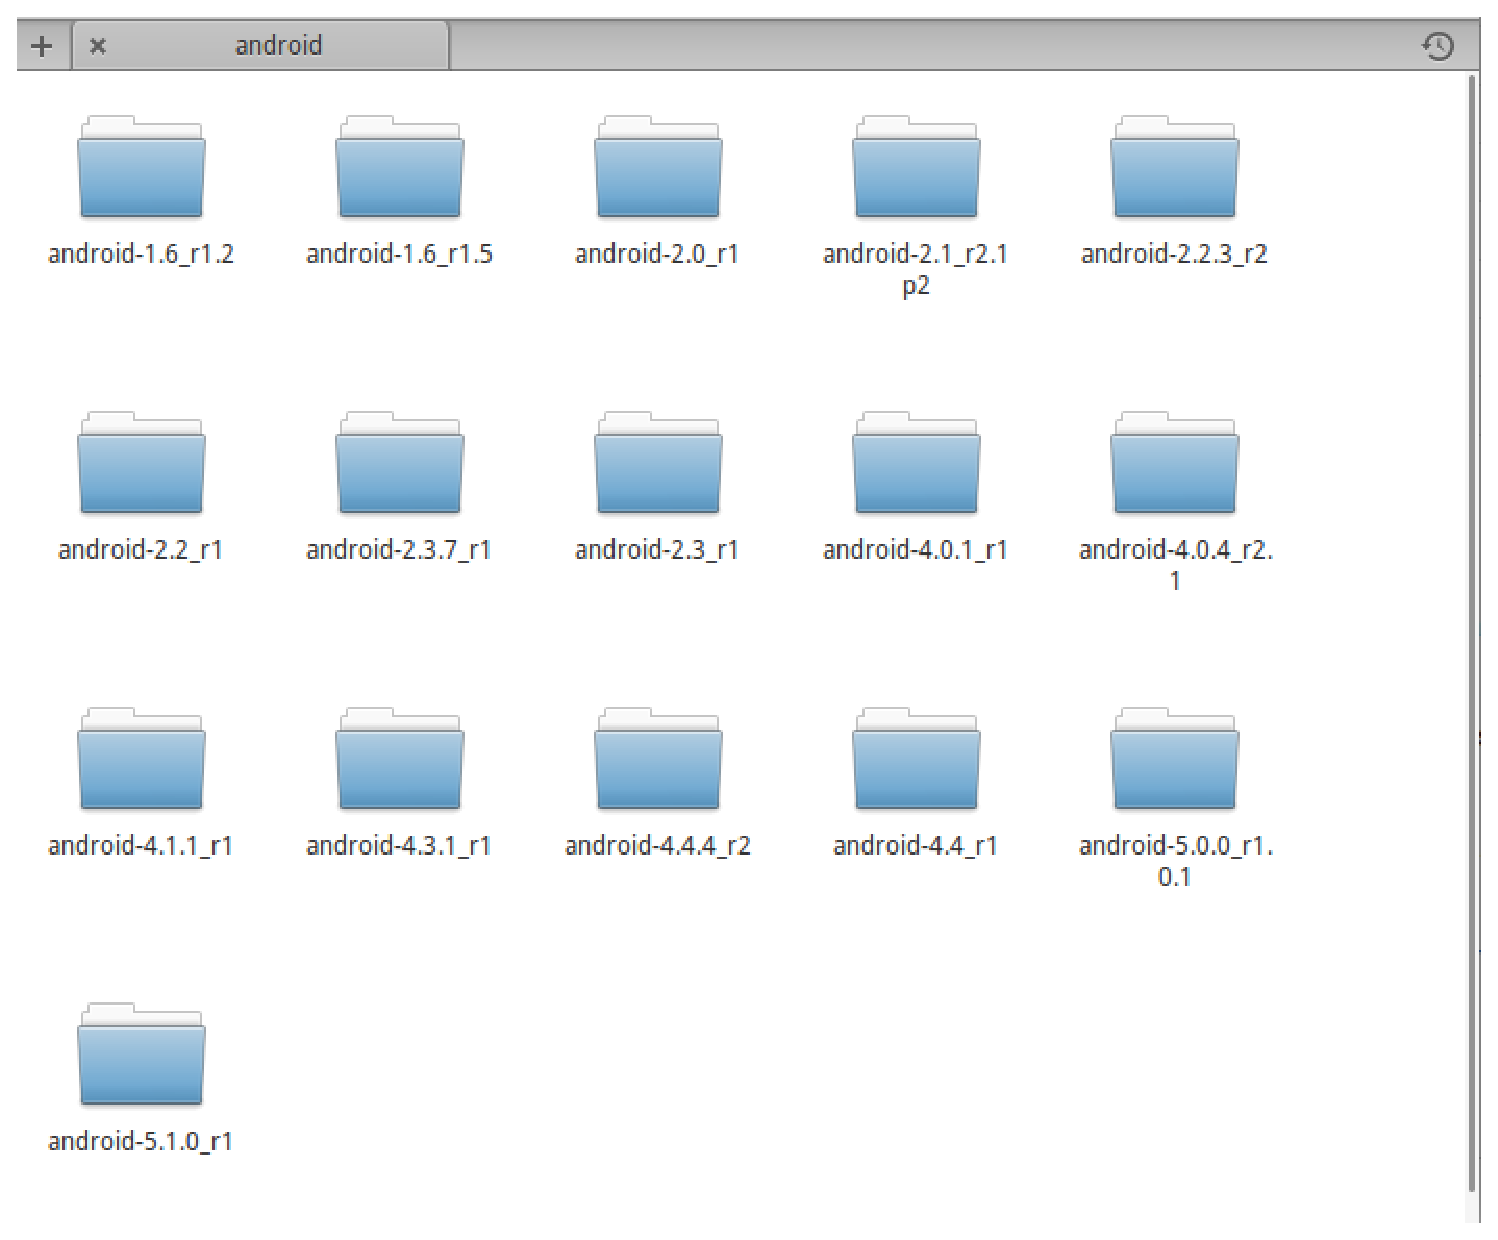
\includegraphics [keepaspectratio=true,scale=0.35]{figuras/folder.eps}
\caption{Diretório onde foram armazenadas cada versão a ser analisada}
\label{folder}
\end{figure}

O restante dos diretórios do AOSP contém desde adaptações de bibliotecas para o Android como o bionic, até código fonte para o \textit{Android Run Time} (ART), que substituiu a dalvik nas ultimas versões do sistema (especificamente desde as versões de \textit{codename Lollipop}), e também códigos de baixo nível específicos para alguns dispositivos. Também existem diretórios para projetos externos ao Android, utilizados pelo mesmo, como o SQLite e outros projetos externos. O kernel utilizado no sistema também tem o seu diretório nessa hierarquia, assim como os aplicativos nativos. A estrutura completa do AOSP não será explorada neste trabalho, mas o conteúdo da pasta raiz pode ser visualizado na Figura~\ref{androidSourceFolders}. A estrutura de diretórios onde foram preparados os códigos para a análise pode ser vista na Figura~\ref{folder}.

Em seguida foi feito o download de cada \textit{tag} em seu diretório, também utilizando a ferramenta \textit{repo}, que realiza um \textit{checkout} de cada subprojeto listado em seu \textit{manifest} através do comando \textit{sync}. O total de espaço em disco ocupado após o download de todas as \textit{tags} foi cerca de 10 GB. É importante notar que esse espaço não corresponde apenas a arquivos de código fonte. Após o download e antes de realizar a análise, foi realizada uma filtragem de arquivos na pasta base da análise, removendo todos os arquivos que não correspondessem a código fonte C, C++ ou Java. Da mesma forma, foram removidos todos os diretórios vazios que restaram da deleção dos arquivos, deixando uma árvore de diretórios menor para ser percorrida pela ferramenta de análise, aumentando assim o desempenho da mesma. O espaço total ocupado pelo código após a filtragem foi de 1,7GB. Não realizar essa remoção não acarretaria em problemas para a análise, entretanto resultaria em um maior tempo necessário para o término da mesma.

Além de todas as versões do Android que foram analisadas, o código fonte dos aplicativos do sistema da ultima versão listada para esta análise (\textit{Android Lollipop} 5.1.0 r1) também foi analisado, com o objetivo principal de comparação com o código do sistema. Aplicativos como de email, calculadora e câmera são analisados pela ferramenta Analizo assim como a API de desenvolvimento. São esperados valores relativos semelhantes aos da API do sistema Android.

%TODO rever porcentagens quando tiver todos os dados
No total foram coletados mais de 100 mil módulos/classes das linguagens C, C++ e Java. Java foi a linguagem mais predominante, com aproximadamente 85\% das amostras, enquanto C++ ocupou pouco mais de 10\% e C pouco mais de 3\%. Embora seja relevante comentar as diferenciações entre as linguagens e seus paradigmas para algumas métricas,  não há necessidade de separação entre os valores para linguagem C, procedural, e linguagens Java/C++, orientadas a objetos, uma vez que, dadas as proporções das mesmas apresentadas nos dados, não há relevância estatística para tal. Entretanto em algumas métricas algumas observações teóricas possam ser ressaltadas, embora, mais uma vez, não haja implicação substancial no resultados gerais apresentados.

\section{Análise de dados}

Após o download de todas as versões escolhidas, foi utilizada a ferramenta Analizo para análise estática de código e coleta de métricas. Foi utilizada a funcionalidade de \textit{batch} do Analizo, de forma a coletar métricas de todas as \textit{tags} de uma só vez. 

O resultado da análise de cada projeto contém os valores parciais das métricas para cada arquivo que foi analisado pela ferramenta. No total são 16 arquivos CSV contendo cada um as métricas para todas as classes/módulos de 1 versão do sistema. O arquivo CSV que contém métricas unificadas para todos os projetos não será utilizado neste trabalho. 

Neste trabalho, serão utilizadas métricas estáticas de código fonte para avaliar a qualidade de um produto de software. Essas métricas utilizadas, essencialmente métricas OO, refletem complexidade arquitetural e decisões de design, como discutido no Capítulo~\ref{cap:metricas}. Métricas de tamanho também serão avaliadas, com o objetivo de relacionar as demais métricas de forma relativa em vez de uma comparação direta, se possível. Métricas de tamanho são mais simples mas ainda são úteis para encontrar problemas arquiteturais no software, como será discutido no Capítulo~\ref{cap:resultados}. Complexidade tem forte relação com o tamanho do código, e manter as duas é uma forma de realizar análises mais adequadas e chegar a resultados mais consistentes.

As métricas finais escolhidas, descritas no Capítulo~\ref{cap:metricas}, foram capturadas pela ferramenta Analizo e estão listadas a seguir:

\begin{itemize}
\item Média de linhas de código por método - \textit{Average Method Lines Of Code} (AMLOC)
\item Média de complexidade ciclomática por método - \textit{Average Cyclomatic Complexity per Method} (ACCM)
\item Resposta para uma classe - \textit{Response For a Class} (RFC)
\item Profundidade na árvore de herança - \textit{Depth in Inheritance Tree} (DIT)
\item Número de subclasses - \textit{Number of Children} (NOC)
\item Falta de coesão em métodos - \textit{Lack of Cohesion in Methods} (LCOM4)
\item Conexões aferentes de uma classe - \textit{Afferent Connections per Class} (ACC)
\item Fator de acoplamento - \textit{Coupling Factor} (COF)
\end{itemize}

Essas métricas foram coletadas para cada classe presente em cada versão do Android analisada. Cada uma das versões contém milhares de classes/módulos a serem computados, e essa grande quantidade de classes ajuda a compensar o pequeno número de versões do sistema que foi utilizado, pois como as métricas são calculadas por classe, foi gerada uma quantidade significativa de amostras para cada tag do sistema.

A maioria das métricas aqui utilizadas foi selecionada por ser bem difundida e discutida na literatura, levando então a ter estudos para relacionar a este. Por exemplo, a possível comparação com valores encontrados em trabalhos semelhantes, como a tese de \citeonline{oliveira2013} e o trabalho de \citeonline{ferreira2009}, incentiva a escolha dessas métricas. Além disso, métricas também úteis, porém não discutidas nesses estudos, como por exemplo as métricas de Halstead, não são capturadas pela ferramenta Analizo.

É importante enfatizar que inicialmente a métrica de acoplamento que seria utilizada seria CBO, a fim de comparação com complexidade estrutural apresentados em trabalhos como o de \citeonline{terceiro2009}. Entretanto, foram encontrados aqui valores muito discrepantes dos valores esperados, divergindo muito dos valores encontrados por \citeonline{meirelles2013}, inclusive para o sistema Android, levando então a conclusão de que algum problema pode ter ocorrido no cálculo da ferramenta. Assim, a métrica de acoplamento utilizada neste estudo foi a métrica ACC.

Para a análise de código fonte em C, que é uma linguagem estruturada, com essas métricas orientadas a objetos, algumas observações devem ser ressaltadas: Em vez de classes, são considerados módulos, e as funções são utilizadas como métodos \cite{terceiro2009}. Embora seja uma abordagem relativamente eficaz para o cálculo das métricas OO, os valores de algumas métricas podem ser bastante distintos das mesmas métricas calculadas para as linguagens que realmente utilizam o paradigma orientado a objetos. Entretanto, como já comentado, não há representatividade da linguagem C nos dados obtidos que motive a análise desses paradigmas isoladamente. Os valores para C++ e Java já se apresentam similares por utilizarem o mesmo paradigma e portanto terem funcionamento semelhante.

Antes de prosseguir com a utilização dos dados, foi preciso executar uma correção dos dados, pois os arquivos CSV de saída continham classes/módulos com parâmetros de tipos genéricos que utilizam vírgula em sua declaração, comprometendo a formatação correta do arquivo CSV, que utiliza vírgula como separador de valores. Esse problema fazia com que algumas linhas fossem calculadas com mais valores do que deveriam conter, uma vez que as vírgulas adicionais empurravam os valores para a direita e os últimos eram então ignorados. A correção de dados então se resumiu em identificar essas amostras que continham vírgulas e remover as vírgulas adicionais. Esses dados corrigidos então foram armazenados em um diretório a parte para utilização nos estágios seguintes.

Após essa captura de todas as métricas, foi utilizada a linguagem R para manipulação inicial dos dados. R é uma linguagem focada computação estatística e possui diversos módulos que facilitam análise estatística, com manipulação facilitada de tabelas e apresentação de dados na forma de gráficos.

Foram calculados, com linguagem R, os percentis de cada métrica para cada versão do sistema analisada. Cada percentil é a centésima parte dos dados ordenados de forma crescente, ou seja, cada percentil contém 1\% dos dados sendo que o primeiro contém as amostras com menor valor. Esses valores representam nada mais que a frequência cumulativa para cada valor. Isso quer dizer que, para o 90º percentil com um valor de 500, por exemplo, 90\% das amostras apresentam o valor menor ou igual a 500. Como essa frequência cumulativa é calculada em cima dos dados ordenados, a mediana pode ser encontrada no 50º percentil.

Os percentis que foram armazenados foram: 1, 5, 10, 25, 50, 75, 90, 95 e 99, além do menor valor e do valor máximo. Esses dados foram posteriormente reunidos em um arquivo em separado para cada métrica contendo os percentis daquela métrica calculados para cada uma das versões do sistema. A Tabela~\ref{exemplo_percentis} contém um exemplo desse resultado demonstrado para a métrica de complexidade ciclomática coletada do código fonte do sistema Android em várias versões, e sua análise será explorada no Capítulo~\ref{cap:resultados}. Os dados coletados para aplicativos foram reunidos da mesma maneira, porém, como só uma versão foi analisada para os aplicativos, em vez de versões, o primeiro valor da tabela é o nome do aplicativo do sistema de onde as métricas foram coletadas.

\begin{table}[!htb]
\centering
\scalefont{.7}
\begin{tabular}{|l|l|l|l|l|l|l|l|l|l|l|l|l|}
\hline
version&classes&min&1\%&5\%&10\%&25\%&50\%&75\%&90\%&95\%&99\%&max\\
\hline
android-1.6\_r1.2&5745&0&0&0&0&1&1.11111111111111&2&3.45454545454545&4.68831967213114&9.5&55\\
\hline
android-1.6\_r1.5&5745&0&0&0&0&1&1.11111111111111&2&3.45454545454545&4.68831967213114&9.5&55\\
\hline
android-2.0\_r1&6331&0&0&0&0&1&1.11111111111111&2&3.5&4.75&9.74444444444443&59\\
\hline
android-2.1\_r2.1p2&6360&0&0&0&0&1&1.11882352941176&2&3.5&4.8&9.88199999999997&60\\
\hline
android-2.2\_r1&7352&0&0&0&0&1&1.06666666666667&2&3.73840579710146&5.2752380952381&12&99\\
\hline
android-2.2.3\_r2&7358&0&0&0&0&1&1.06666666666667&2.01744186046512&3.75&5.26173913043478&12&99\\
\hline
android-2.3\_r1&8093&0&0&0&0&1&1&2.07142857142857&4&5.81691176470588&12.8275&99\\
\hline
android-2.3.7\_r1&8240&0&0&0&0&1&1&2.08333333333333&4&5.8&12.755625&99\\
\hline
android-4.0.1\_r1&11709&0&0&0&0&1&1&2.125&4&6&17&94.3333333333333\\
\hline
android-4.0.4\_r2.1&11851&0&0&0&0&1&1&2.10858585858586&4&6&17&94.3333333333333\\
\hline
android-4.1.1\_r1&14115&0&0&0&0&1&1&2&3.85631469979296&5.77846153846152&16&99.4\\
\hline
android-5.1.0\_r1&20129&0&0&0&0&1&1&2&3.5&5&11&158.6\\
\hline
\end{tabular}

\caption{Complexidade ciclomática nas versões da API analisadas}
\label{exemplo_percentis}
\end{table} 

Com esses arquivos em mãos com os valores de vários percentis para cada métrica nas diversas versões, podem então ser gerados gráficos para melhor visualizar a evolução de cada métrica juntamente com a evolução do sistema. Esses resultados serão discutidos no Capítulo~\ref{cap:resultados}.

Alguns outros gráficos também podem ser gerados a partir dos dados completos, com os valores de cada métrica para cada classe. Gráficos como de distribuição, demonstrando os valores mais frequentes, e gráfico de linha ou de área para demonstrar evolução das métricas, são bastante úteis para a análise dos dados coletados. 

Assim como feito por ~\citeonline{meirelles2013}, os resultados das análises discutidos no Capítulo~\ref{cap:resultados} serão em função dos percentis 75, 90 e 95, correspondendo a valores muito frequentes, frequentes e pouco frequentes, respectivamente. A utilização de 95\%, embora não inclua todas as amostras, ainda resulta em uma boa amostra estatística, uma vez que, como os valores estão ordenados, boa parte desses 5\% restantes são valores discrepantes que podem interferir negativamente na análise correta dos dados.

Este capítulo teve o intuito de descrever os procedimentos gerais para obtenção e análise dos dados, enquanto a análise em si será abordada no Capítulo~\ref{cap:resultados}. Ainda no capítulo de resultados, será apresentada uma proposta a verificação de similaridade de aplicativos em relação à API, com base nos valores dessas métricas coletadas e nas distribuições dos valores a partir dos percentis 75, 90 e 95. São apresentadas discussões sobre grandeza dos dados das métricas, normalização de valores, e uma abordagem de pesos para dar às métricas diferentes valores de importância no valor final de similaridade. É importante ressaltar que esse cálculo que será feito não resulta em um valor com significado semântico relacionado ao seu valor absoluto, pois o mesmo não tem uma medida, e portanto será utilizado apenas em comparação com os valores de similaridade calculados para outros aplicativos e verificação de distancia do valor de referência da API, representado pelo número 0. Uma fórmula para cálculo desse valor é apresentada para que outros projetos possam ter sua distância calculada e poder fazer comparação com os resultados dessa proposta.
